
During the development of this work, many experiments were conducted before reaching the main objective. To provide a better understanding of the chosen approach and to contribute to future research by highlighting different methods and their outcomes, a summary of each experiment and its corresponding results is presented below.

\section{Experiment 1}

Use of a Multilayer Neural Network to analyze the audio input (in the time domain) and estimate the corresponding FM synthesis parameters in order to resynthesize the audio. Main highlights:

\begin{enumerate}
\item 1000 audio input samples (each 3 seconds long).
\item Each audio input was split into frames of 2048 samples (resulting in 43 frames per audio sample).
\item The neural network was divided into two parts: the first acted as a feature extractor (with a time-distributed layer using three deep layers); the second was a regressor, consisting of a more conventional neural network (with tree layers) used to estimate the FM synthesis parameters based on the previously extracted audio features.
\item The results were poor, and the model suffered from overfitting (despite testing many variations).
\end{enumerate}

The network architecture is presented below:

\begin{figure}[htb]
 \caption{Experiment 1 architecture}
 \label{fig:experiment1_arch}
 \centering
 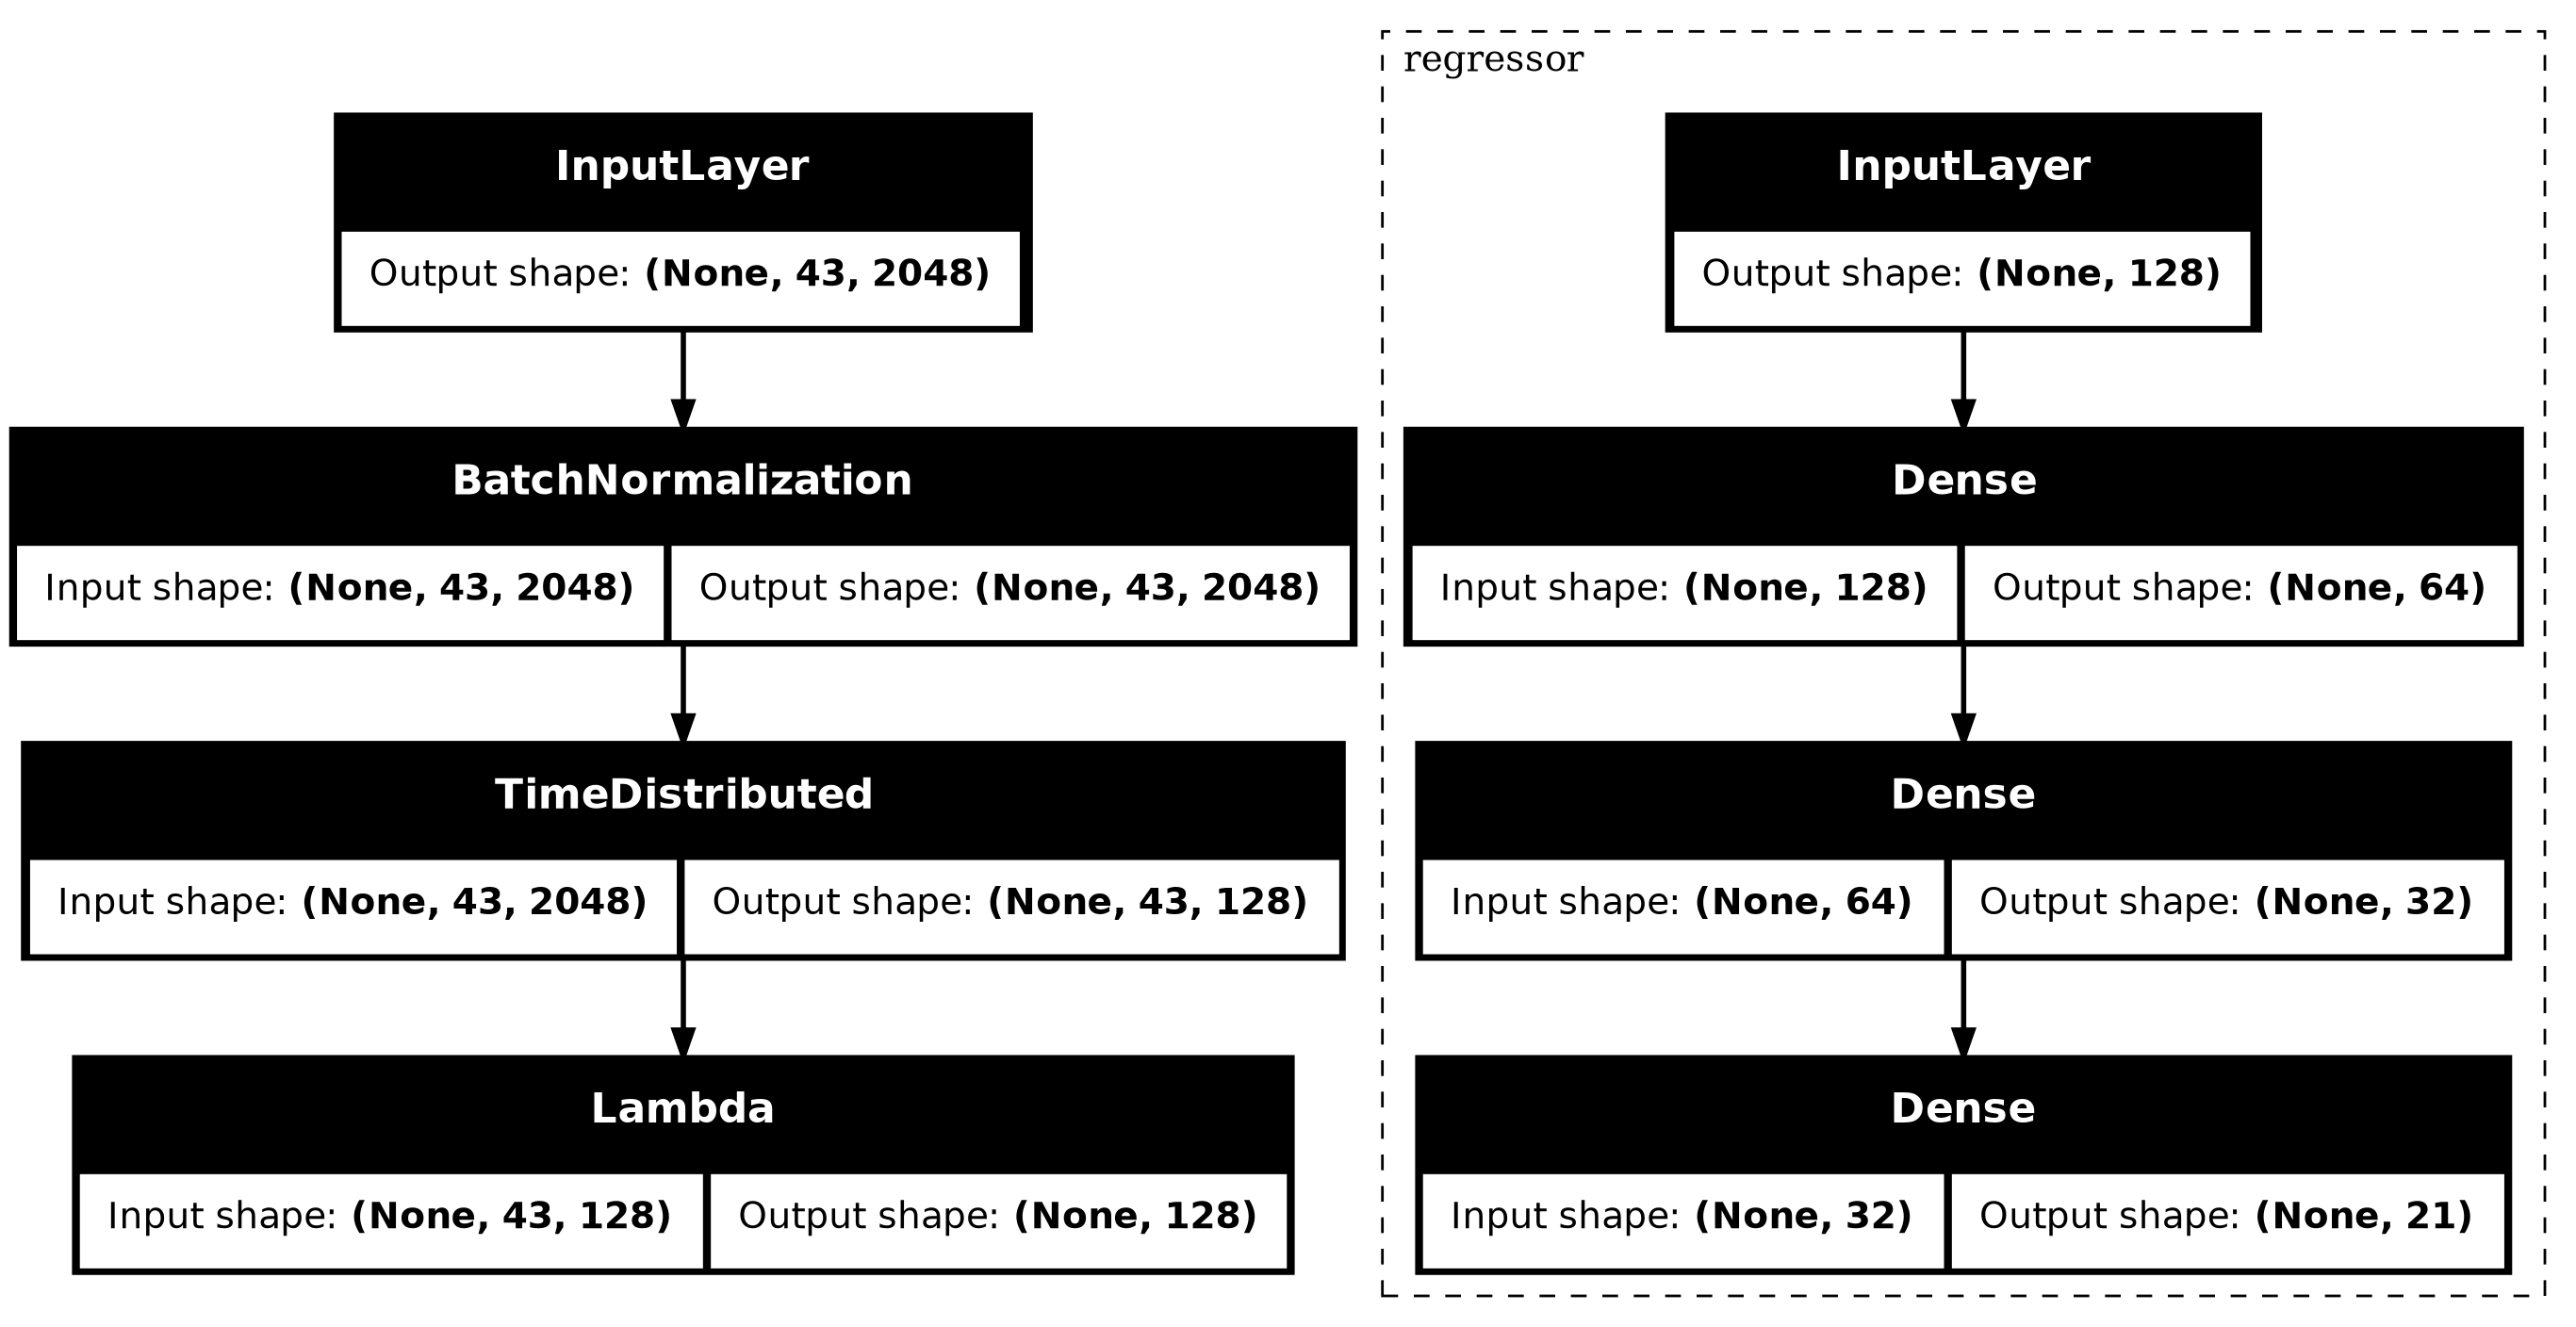
\includegraphics[scale=0.15]{images/experiment1.png}
 \fdireta{usp:logo}
\end{figure}

Summary of the evaluation metrics from the training process:

\begin{figure}[htb]
 \caption{Experiment 1 MSE error}
 \label{fig:experiment1_mse}
 \centering
 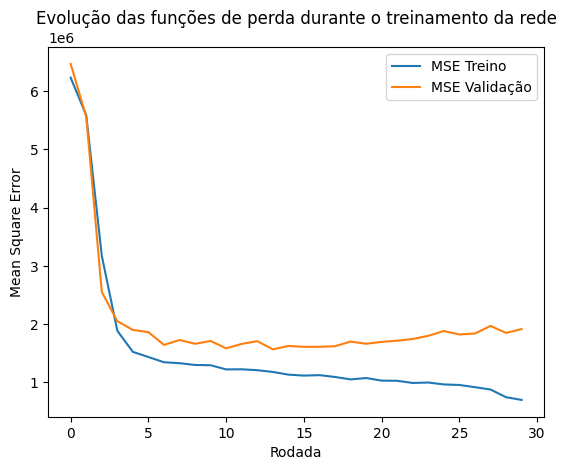
\includegraphics[scale=1]{images/experiment1_mse.png}
 \fdireta{usp:logo}
\end{figure}

\begin{figure}[htb]
 \caption{Experiment 1 MAE error}
 \label{fig:experiment1_mae}
 \centering
 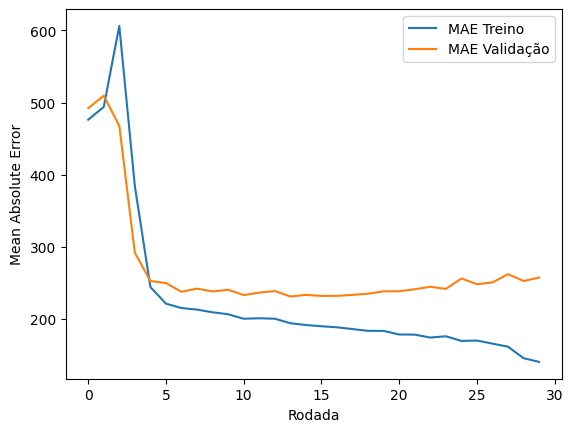
\includegraphics[scale=1]{images/experiment1_mae.png}
 \fdireta{usp:logo}
\end{figure}

\section{Experiment 2}

Use of a 1D Convolutional Neural Network to extract audio features from the time-domain representation, and to estimate the corresponding FM synthesis parameters using a standard Multilayer Neural Network. Main highlights:

\begin{enumerate}
\item 1000 audio input samples (each 1 second long, to avoid memory exhaustion).
\item The audio inputs were not further split into frames.
\item The neural network was divided into two parts: the first acted as a feature extractor, consisting of three convolutional layers; the second was a regressor, made up of a conventional neural network (with three layers) used to estimate the FM synthesis parameters based on the previously extracted audio features.
\item The results were better than in previous experiments, but still poor. Moreover, the model suffered from even more intense overfitting (despite testing many variations).
\end{enumerate}

The network architecture is presented below:

\begin{figure}[htb]
 \caption{Experiment 2 architecture}
 \label{fig:experiment2_arch}
 \centering
 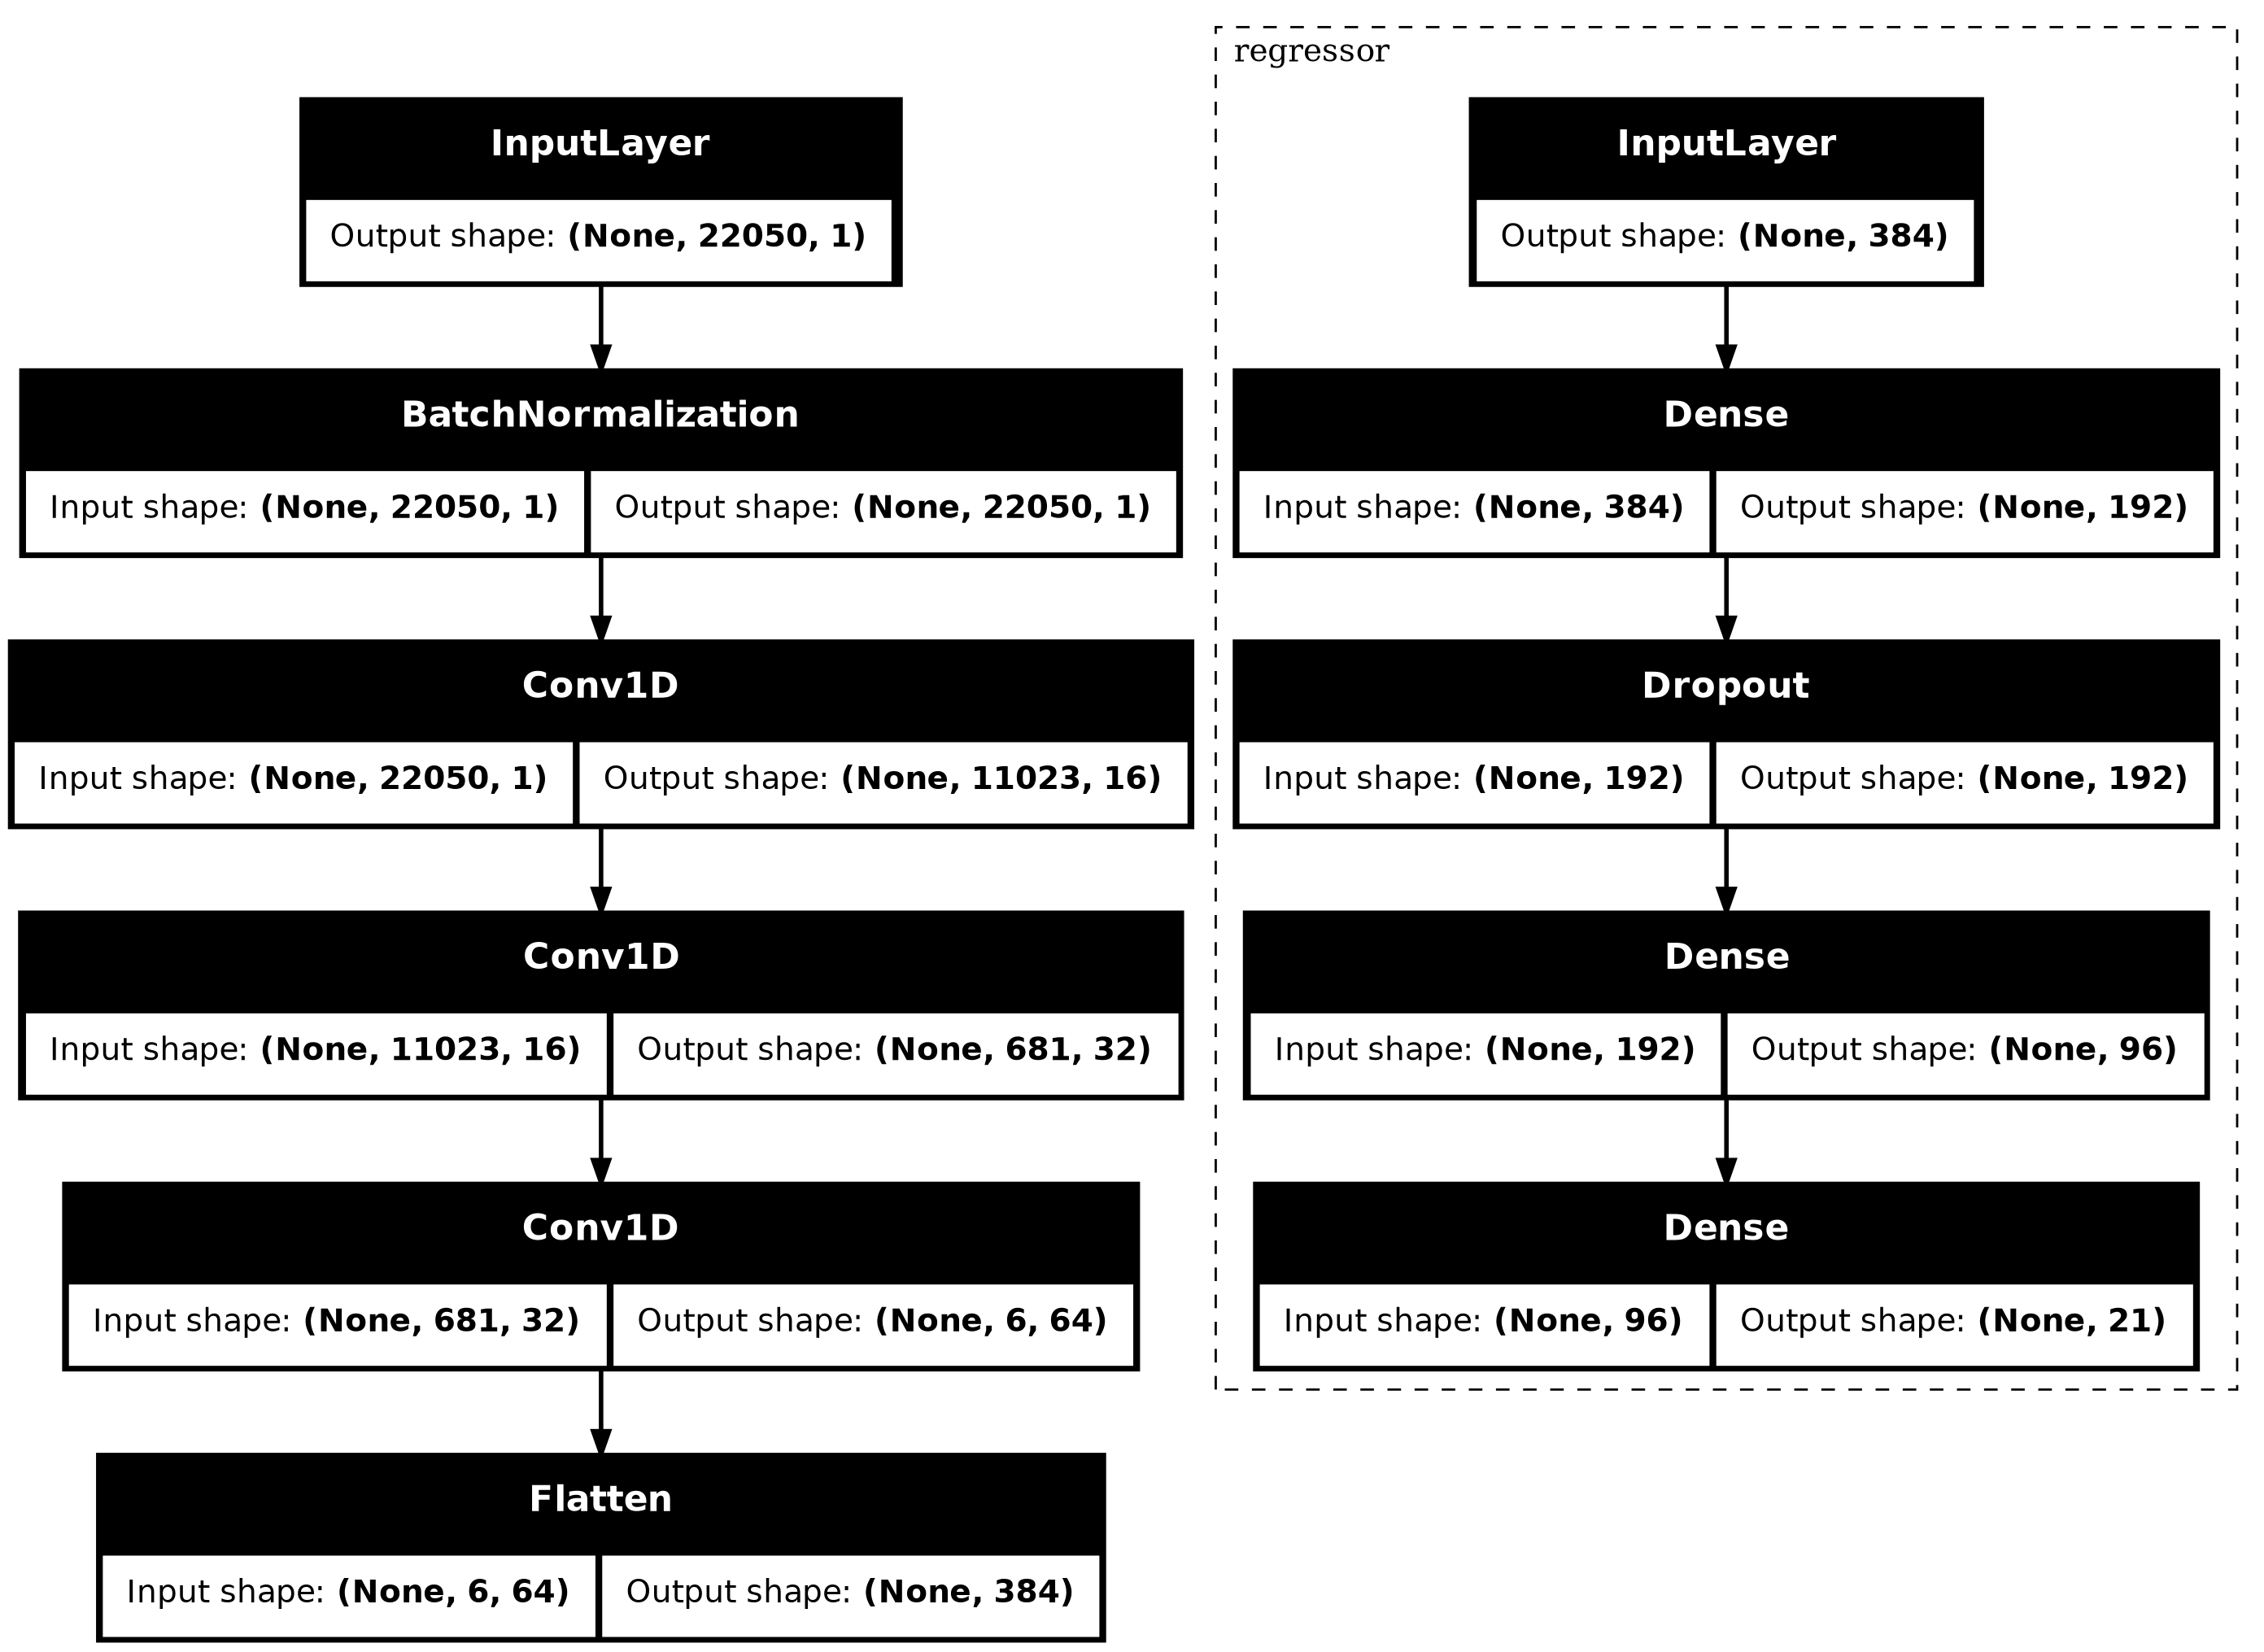
\includegraphics[scale=0.18]{images/experiment2.png}
 \fdireta{usp:logo}
\end{figure}

Summary of the evaluation metrics from the training process:

\begin{figure}[htb]
 \caption{Experiment 2 MSE error}
 \label{fig:experiment2_mse}
 \centering
 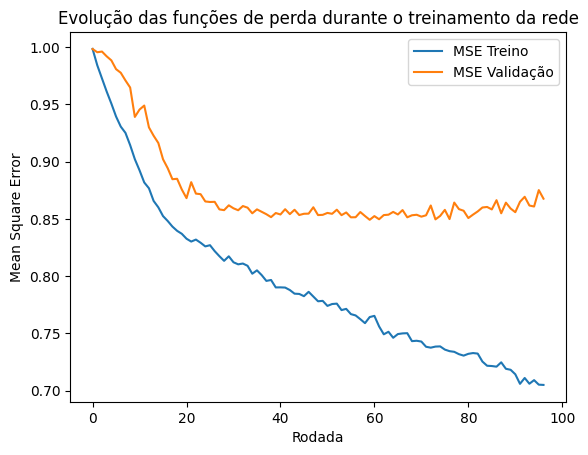
\includegraphics[scale=1]{images/experiment2_mse.png}
 \fdireta{usp:logo}
\end{figure}

\begin{figure}[htb]
 \caption{Experiment 2 MAE error}
 \label{fig:experiment2_mae}
 \centering
 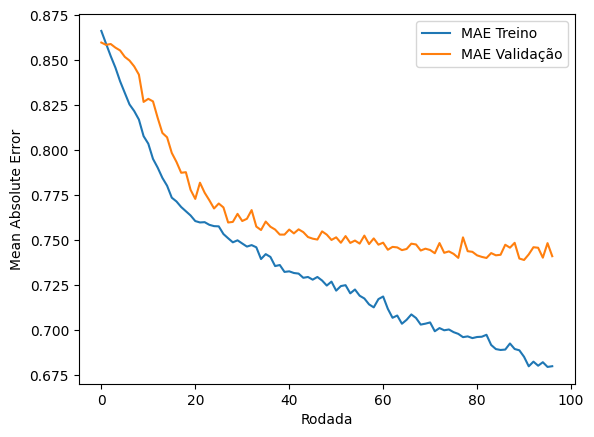
\includegraphics[scale=1]{images/experiment2_mae.png}
 \fdireta{usp:logo}
\end{figure}

\section{Experiment 3}

Very similar to the Experiment 2, but, with one convolutional layer less, but adding MaxPooling layers, on the extractor network.

\begin{enumerate}
\item 1000 audio input samples (each 1 second long, to avoid memory exhaustion).
\item The neural network was divided into two parts: the first acted as a feature extractor, consisting of three convolutional layers, plus poolgin layers; the second was a regressor, made up of a conventional neural network (with three layers) used to estimate the FM synthesis parameters based on the previously extracted audio features.
\item The results were similar to the previous experiments.
\end{enumerate}

The network architecture is presented below:

\begin{figure}[htb]
 \caption{Experiment 3 architecture}
 \label{fig:experiment3_arch}
 \centering
 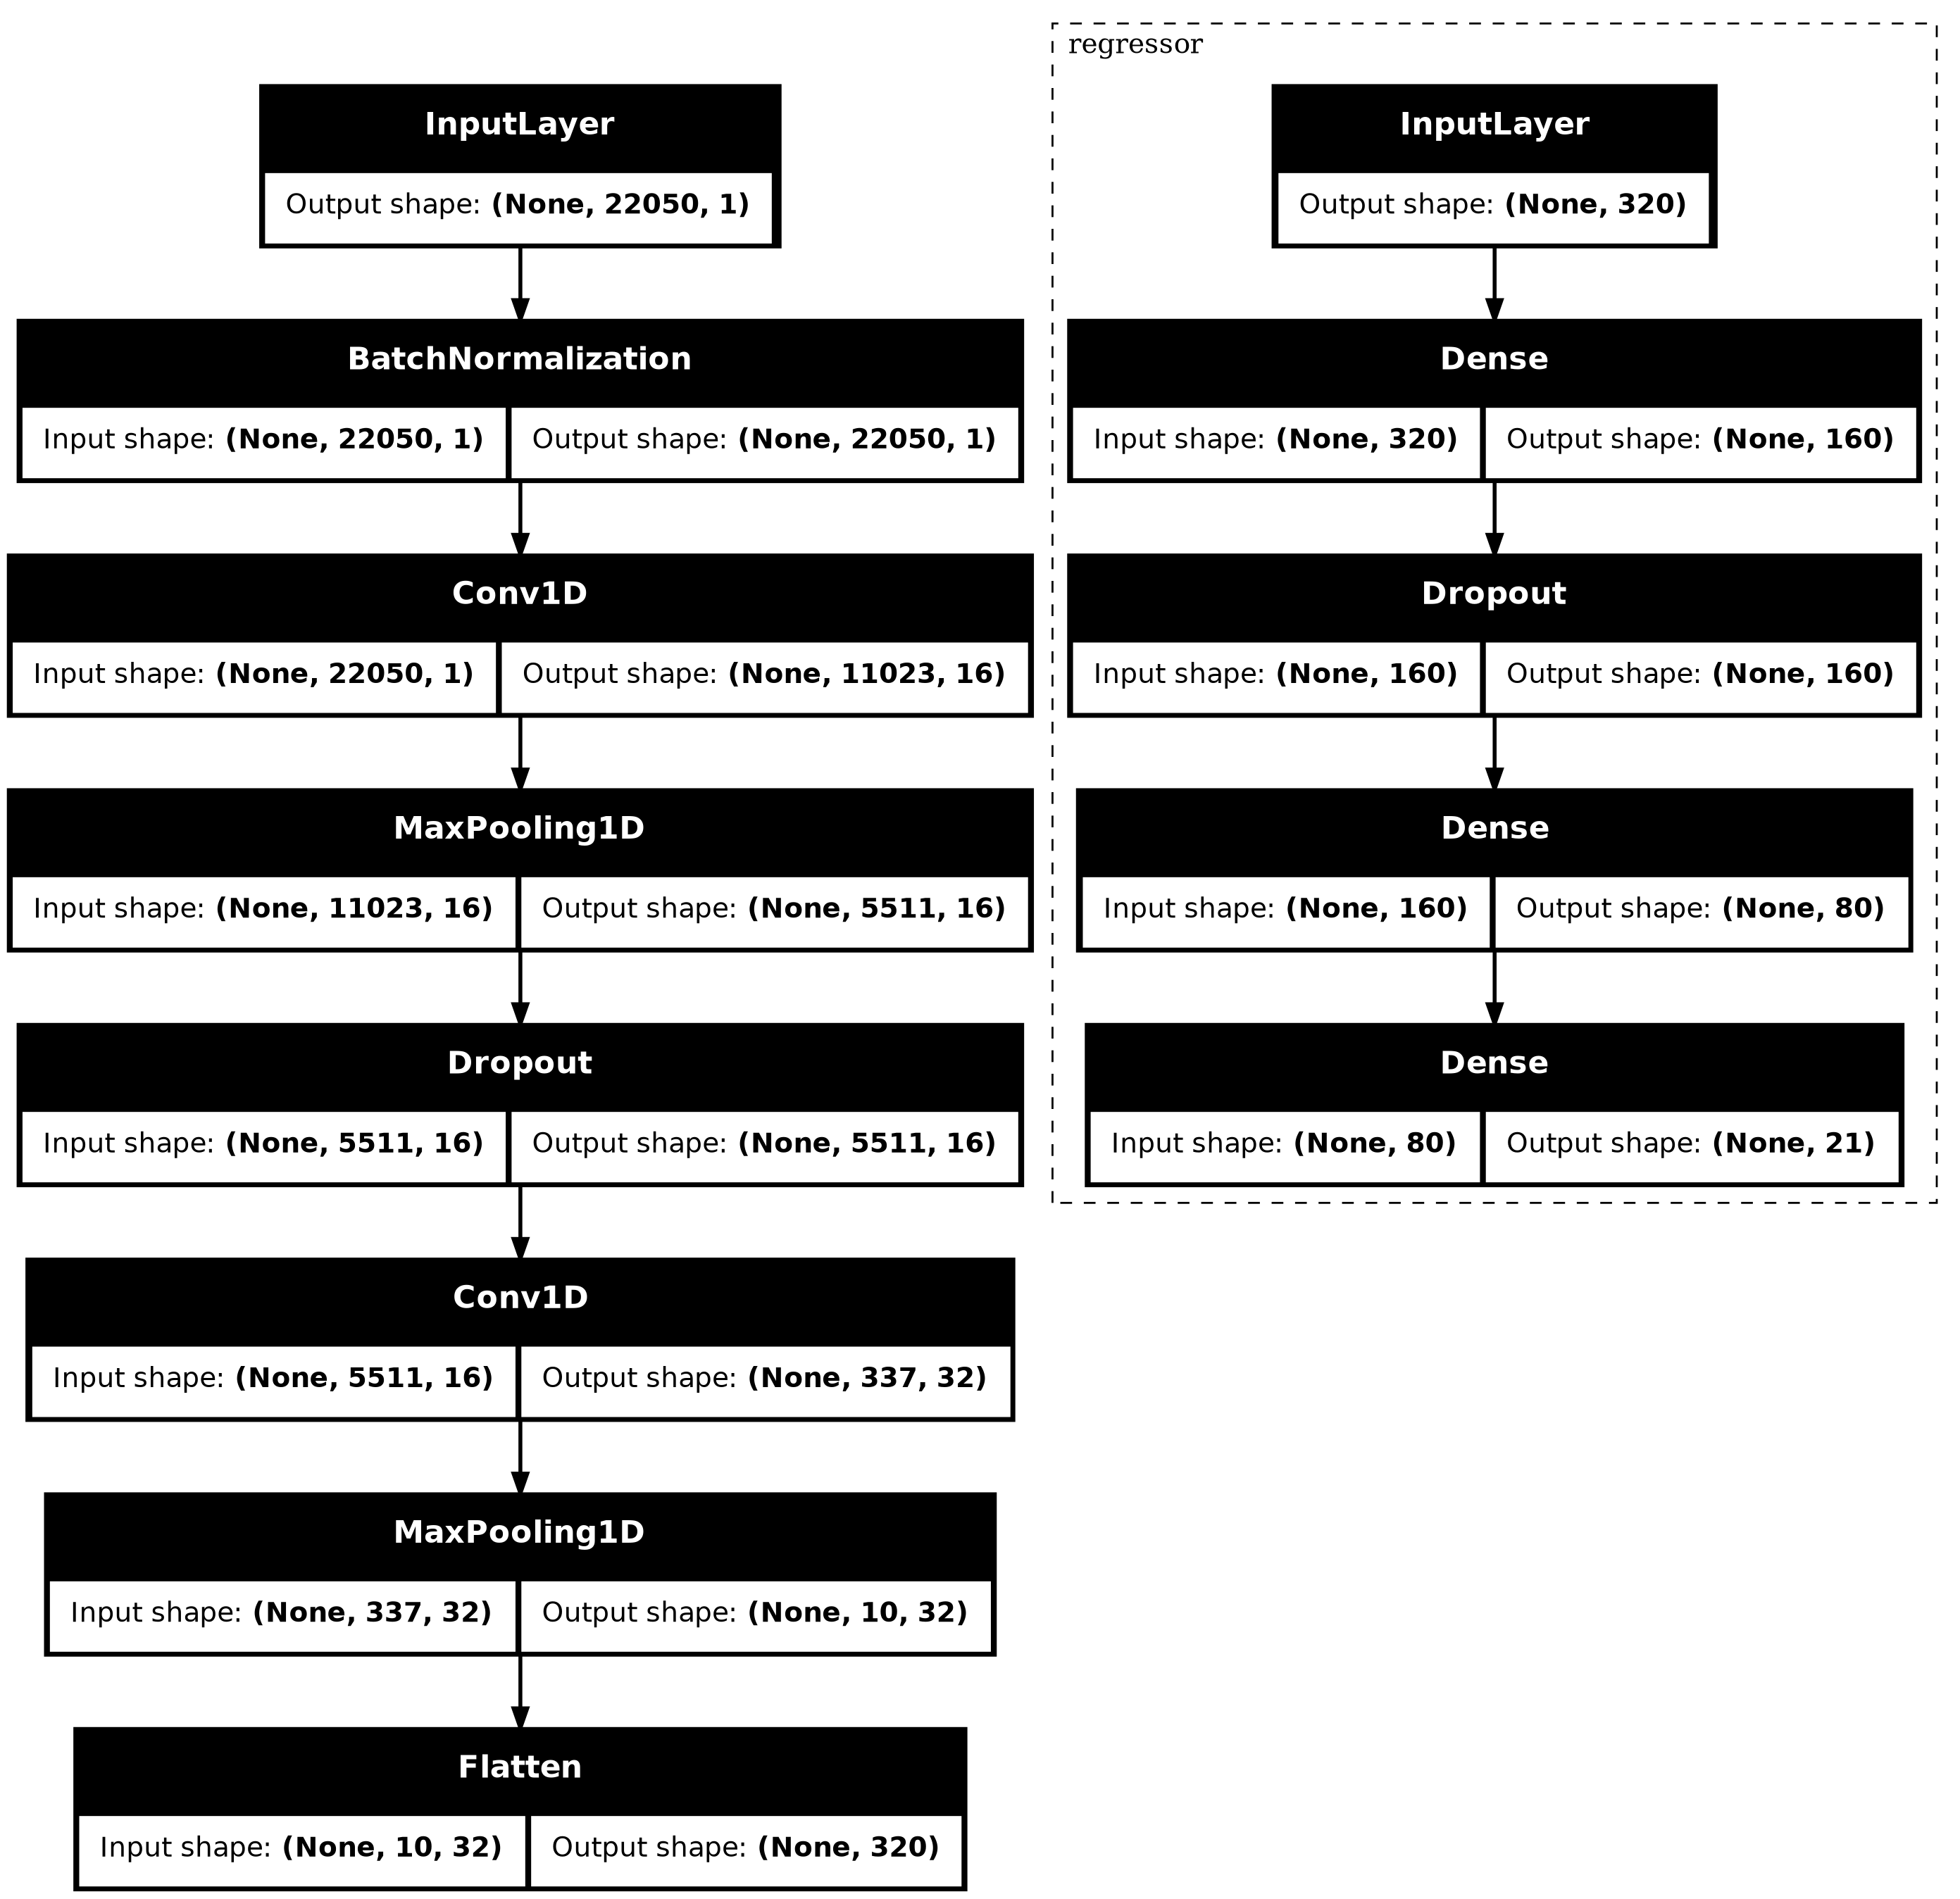
\includegraphics[scale=0.18]{images/experiment3.png}
 \fdireta{usp:logo}
\end{figure}

Summary of the evaluation metrics from the training process:

\begin{figure}[htb]
 \caption{Experiment 3 MSE error}
 \label{fig:experiment3_mse}
 \centering
 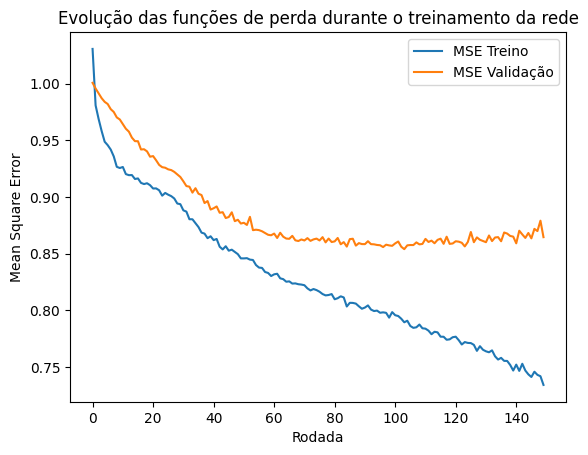
\includegraphics[scale=1]{images/experiment3_mse.png}
 \fdireta{usp:logo}
\end{figure}

\begin{figure}[htb]
 \caption{Experiment 3 MAE error}
 \label{fig:experiment3_mae}
 \centering
 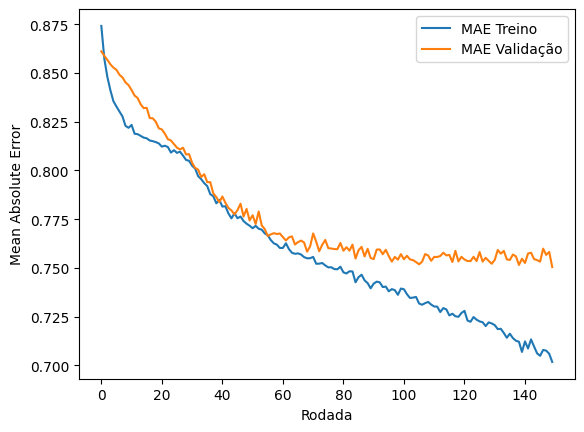
\includegraphics[scale=1]{images/experiment3_mae.png}
 \fdireta{usp:logo}
\end{figure}

\section{Experiment 4}

This experiment is very similar to Experiments 2 and 3, but with two branches of convolutional layers in the feature extraction part of the model.

Here, pooling layers are also used. The main idea is to apply different filters and pooling strategies in each branch, in order to capture distinct features and recognize different frequency patterns in the audio input.

The regression model remains similar to the previous experiments.

\begin{enumerate}
\item 1000 audio input samples (each 1 second long, to avoid memory exhaustion).
\item The neural network was divided into two main parts: a feature extractor and a regressor. However, the feature extractor itself was composed of two parallel convolutional branches.
\item The results were slightly worse than in the previous experiment, but still similar. However, this time, the model did not suffer from overfitting.
\end{enumerate}

The network architecture is presented below:

\begin{figure}[htb]
 \caption{Experiment 4 architecture}
 \label{fig:experiment4_arch}
 \centering
 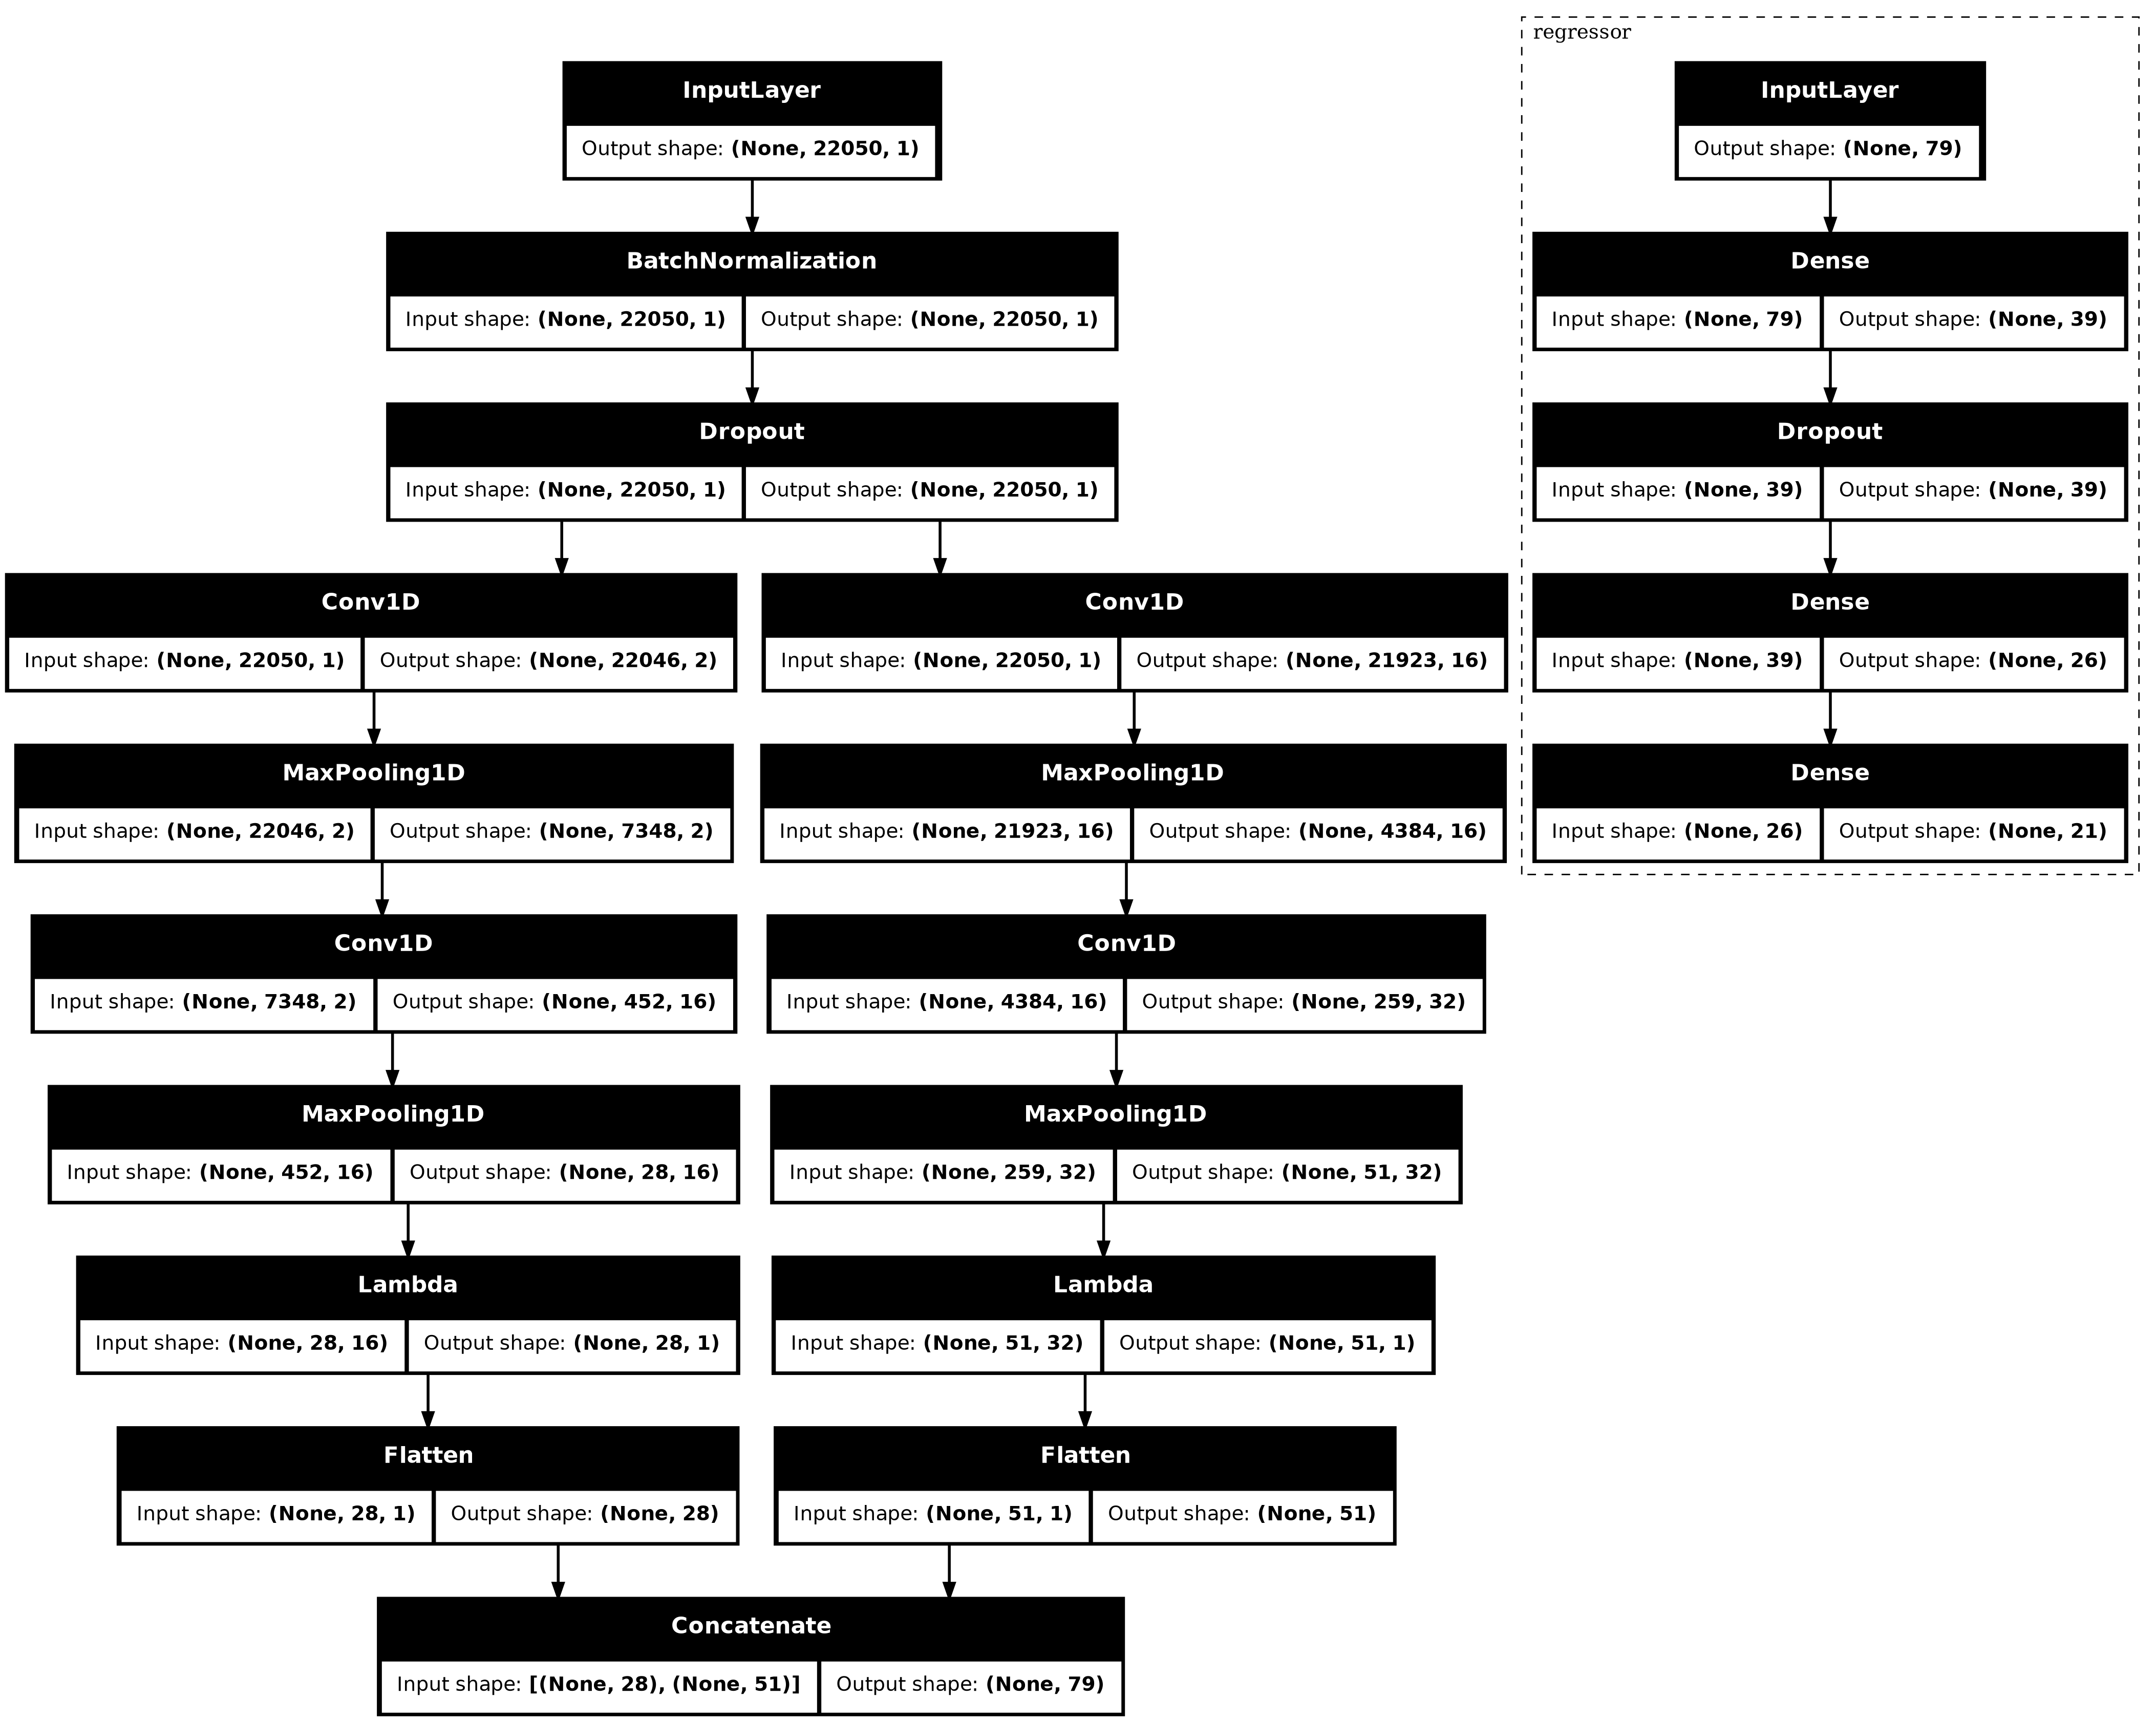
\includegraphics[scale=0.11]{images/experiment4.png}
 \fdireta{usp:logo}
\end{figure}

Summary of the evaluation metrics from the training process:

\begin{figure}[htb]
 \caption{Experiment 4 MSE error}
 \label{fig:experiment4_mse}
 \centering
 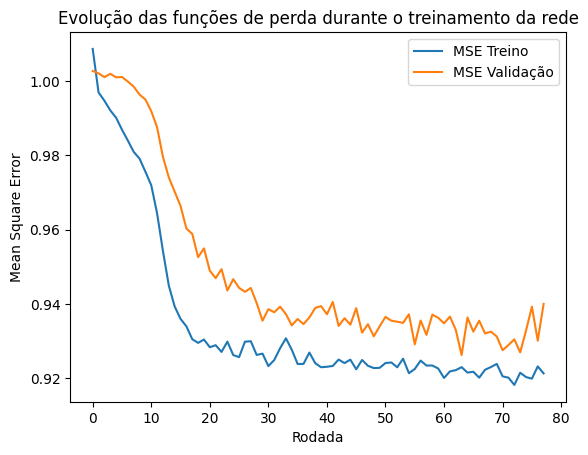
\includegraphics[scale=1]{images/experiment4_mse.png}
 \fdireta{usp:logo}
\end{figure}

\begin{figure}[htb]
 \caption{Experiment 4 MAE error}
 \label{fig:experiment4_mae}
 \centering
 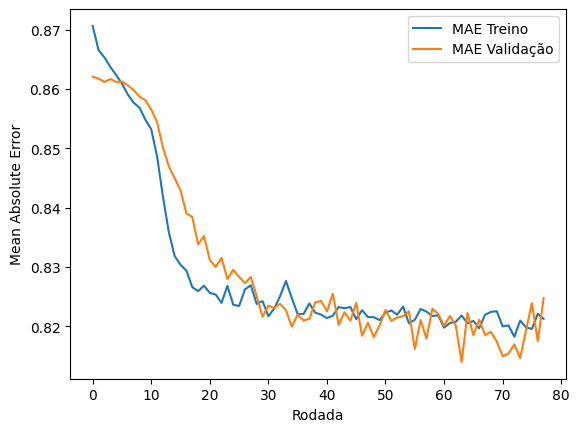
\includegraphics[scale=1]{images/experiment4_mae.png}
 \fdireta{usp:logo}
\end{figure}
